\documentclass[11pt]{article}
\usepackage[hmargin=1in,vmargin=1in]{geometry}
\usepackage{xcolor}
\usepackage{amsmath,amssymb,amsfonts,url,sectsty,framed,tcolorbox,framed}
\usepackage{nicematrix}
\setcounter{MaxMatrixCols}{16}
\usepackage{tikz}
\usepackage{hyperref}
\usetikzlibrary{decorations.pathreplacing}
\newcommand{\pf}{{\bf Proof: }}
\newtheorem{theorem}{Theorem}
\newtheorem{lemma}{Lemma}
\newtheorem{proposition}{Proposition}
\newtheorem{definition}{Definition}
\newtheorem{remark}{Remark}
\newcommand{\qed}{\hfill \rule{2mm}{2mm}}


\begin{document}
%%%%%%%%%%%%%%%%%%%%%%%%%%%%%%%%%%%%%%%%%%%%%%%%%%%%%%%%%%%%%%%%%%%%%
\noindent
\rule{\textwidth}{1pt}
\begin{center}
{\bf [CS304] Introduction to Cryptography and Network Security}
\end{center}
Course Instructor: Dr. Dibyendu Roy \hfill Winter 2022-2023\\
Scribed by: Archit Agrawal (202051213) \hfill Lecture 5 and 6 (Week 3)
\\
\rule{\textwidth}{1pt}
%%%%%%%%%%%%%%%%%%%%%%%%%%%%%%%%%%%%%%%%%%%%%%%%%%%%%%%%%%%
%write here

\section{Quick Recap}
In the second week, the following topics were covered:
\begin{itemize}
    \item Classical Ciphers: Playfair, Hill and Substitution Cipher
    \item Kerkchoff's Principle and Shannon's Notion of Perfect Secrecy
    \item Symmetric Key Cipher: Block and Stream Cipher
    \item Product Cipher: Substitution Permutation Network
    \item Feistel Network
    \item Iterated Block Cipher 
    \item One Time Padding 
\end{itemize}


\section{One Time Padding}
One Time Padding (OTP) provides perfect secrecy under some conditions.\\
\newline
\textbf{Encryption: }
\begin{center}
    P $\rightarrow$ Plain Text\\
    K $\rightarrow$ Secret Key\\
    $Enc(P, K) = P \oplus K = C$\\
    $\oplus \rightarrow $ xor operation\\
\end{center}
\textbf{Decryption: }
\begin{center}
    $Dec(C, K) = C \oplus K = P$\\
\end{center}
The conditions under which OTP provides perfect secrecy are as follows:
\begin{enumerate}
    \item The secret key K cannot be used to encrypt two messages, that is, the key can not be reused.
    \item The length of key must be greater than or equal to the length of message.
    \item Key K is uniformly selected from the key space.
\end{enumerate}
Stream Cipher is a generalisation of OTP which does not provide perfect secrecy.

\subsection{OTP on One Bit Encryption}
The message and key will be of one bit. The probabilities of the message and keys are mentioned below:
\begin{center}
    $Pr[m = 0] = p$\\
    $Pr[m = 1] = 1 - p$\\
    $Pr[k = 0] = 0.5$\\
    $Pr[k = 1] = 0.5$\\
\end{center}
where m is one bit message $(m \in \{0, 1\})$ and k $(k \in \{0, 1\})$ is one bit key.
Since, key is to be chosen uniformly, hence, its probability is 0.5 for values 0 and 1.\\
\textbf{Encryption: } C = m $\oplus$ k\\
\newline
Cipher text can be 0 or 1. Let us find the probability of cipher text to be zero.
\begin{center}
    Pr[C = 0] = Pr[m = 0, k = 0] + Pr[m = 1, k = 1]
\end{center}
The events [m = 0, k = 0] and [m = 1, k = 1] are mutually exclusive gives the cipher text 0. Hence, probability of cipher text to be zero is summation of both these probabilities. Also, the message bits and the key bits are independent of each other, that is, the value of one doesn't affect the other in any way. Hence, the above equation can be written as:

\begin{center}
    $Pr[C = 0] = Pr[m = 0] \cdot Pr[k = 0] + Pr[m = 1] \cdot Pr[k = 1]$\\
    $Pr[C = 0] = p \cdot 0.5 + (1 - p) \cdot 0.5$\\
    $Pr[C = 0] = 0.5$
\end{center}
Similarly, it can be found that Pr[C = 1] = 0.5. To prove that OTP provides perfect secrecy, we need to prove the following statement:
\begin{center}
    $Pr[M = m | C = c] = Pr[M = m]$
\end{center}
We know that:
\begin{center}
    $Pr[A|B] = \frac{Pr[AB]}{Pr[B]}$\\
    $Pr[AB] = Pr[B|A] \cdot Pr[A]$
\end{center}
Therefore, 
\begin{center}
    $Pr[m = 0 | c = 0] = \frac{Pr[m = 0, c = 0]}{Pr[c = 0]} $\\
\end{center}
\begin{center}
    $Pr[m = 0 | c = 0] = \frac{Pr[c = 0 | m = 0] \cdot Pr[m = 0]}{Pr[c = 0]} $
\end{center}
If the cipher text is 0, given that the message is 0, then key can have only one possible value (e.g. 0), which means:
\begin{center}
    $Pr[c = 0 | m = 0] = Pr[k = 0] = 0.5$\\
    $\therefore Pr[m = 0 | c = 0] = \frac{0.5 \cdot Pr[m = 0]}{0.5}$
\end{center}
\begin{center}
    Pr[m = 0 | c = 0] = Pr[m = 0]
\end{center}
Hence, the equation for perfect secrecy is proved under the conditions that were mentioned earlier. The proof can be generalized for any number of bits. \\
\newline
In the proof above, we took the length of key equal to the message and the key to be uniformly selected from key space by assigning equal probability of 0.5. Now, lets try to understand what will happen if same key is used to encrypt two messages.
\begin{center}
    $M_1 \oplus k = C_1$\\
    $M_2 \oplus k = C_2$
\end{center}
$M_1$ and $M_2$ are two messages encrypted using the same key and we have only the cipher text $C_1$ and $C_2$. 
\begin{center}
$C_1 \oplus C_2 = (M_1 \oplus k) \oplus (M_2 \oplus k)$\\
$C_1 \oplus C_2 = M_1 \oplus M_2$
\end{center}
Xoring the cipher texts gives us some additional knowledge about the messages. Let's say $C_1 \oplus C_2 = 00..101$. This states that the MSB's of the two messages $M_1$ and $M_2$ are same while their LSB's are different. That is, the difference in cipher text will reveal the difference in messages.\\
\newline
Now, lets understand what will happen when length of key is strictly lesser than length of message. Let's say there is a 32 bit message and a 16 bit key. Now, to make XOR operation possible, the key must become at least equal to the length of message. There are several ways this can be done, two of them are mentioned below:
\begin{enumerate}
    \item Add 16 0's or 1's in the key, maybe as LSB or MSB.
    \begin{center}
        key: 0000 0000 0000 0000 k
    \end{center}
    where k is actual 16 bit key. The problem here is that 16 bits of the message will not be encrypted only. That is, we will get 16 bits of message without any encryption in the cipher text.

    \item The other way is to repeat a certain number of key bits and add them either as LSB or MSB.
    \begin{center}
        $P = P_1P_2.........P_n$\\
        $K = K_1K_2....K_lK_1K_2....K_t$
    \end{center}
    where, $n = l + p$, n is length of message, t is length of key $(t < n)$ and first l bits of key are used again.
    \begin{center}
        $C = (P_1 \oplus K_1)(P_2 \oplus K_2)...(P_l \oplus K_l)(P_{l+1} \oplus K_1)...(P_n \oplus K_t)$\\
        $C = C_1C_2....C_lC_{l+1}....C_n$
    \end{center}
    Now, if we perform $C_1 \oplus C_{l+1}$, we will get $(P_1 \oplus P_{l+1})$. Hence, cipher text will reveal the difference between first and $(l+1)^{th}$ bit of the message.
\end{enumerate}
One Time Padding with above conditions satisfying, i.e. providing perfect secrecy, is not usable in practical life. This is because for communication the key will be different every time and also length of key will be as long as (if not more) the message. This means that there will be a mechanism to share the secret key securely. Hence, the same mechanism can be used to communicate the message, rather than the security key.

\section{Data Encryption Standard (DES)}
Data Encryption Standard is a block cipher designed by IBM. It is based on Feistel Networks. It has the following parameters:
\begin{itemize}
    \item Block Size = 64 bits
    \item Number of Rounds = 16
    \item Secret Key Size = 64 bits (8 parity check bits)
\end{itemize}
Initially, the design was kept secret and it was used for personal communication only. But when the design came into the public domain, immediately the cipher was broken. There are several weaknesses which reveals the secret key in a quick time.\\
\newline 
The actual secret key is if 56 bits. The 8 parity bits depends on the 56 bits of the key. The parity bits ensure if the other bits are correct or not.To find the secret key of DES exhaustively, $2^{56}$ keys will be checked in the worst case.\\
\newline
\textbf{Encryption: }
\begin{center}
    \tikzset{every picture/.style={line width=0.75pt}}  
    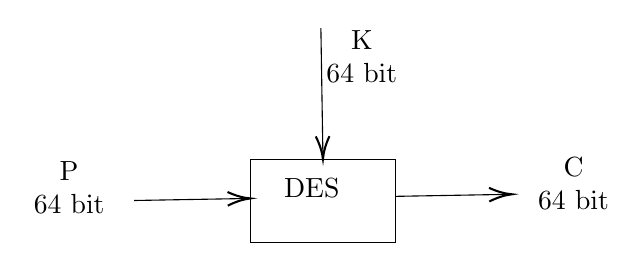
\begin{tikzpicture}[x=0.75pt,y=0.75pt,yscale=-1,xscale=1]
        \draw   (263,99) -- (333,99) -- (333,139) -- (263,139) -- cycle ;
        \draw    (297,35.8) -- (297.97,96.8) ;
        \draw [shift={(298,98.8)}, rotate = 269.09] [color={rgb, 255:red, 0; green, 0; blue, 0 }  ][line width=0.75]    (10.93,-3.29) .. controls (6.95,-1.4) and (3.31,-0.3) .. (0,0) .. controls (3.31,0.3) and (6.95,1.4) .. (10.93,3.29)   ;
        \draw    (207,118.8) -- (261,117.84) ;
        \draw [shift={(263,117.8)}, rotate = 178.98] [color={rgb, 255:red, 0; green, 0; blue, 0 }  ][line width=0.75]    (10.93,-3.29) .. controls (6.95,-1.4) and (3.31,-0.3) .. (0,0) .. controls (3.31,0.3) and (6.95,1.4) .. (10.93,3.29)   ;
        \draw    (333,116.8) -- (387,115.84) ;
        \draw [shift={(389,115.8)}, rotate = 178.98] [color={rgb, 255:red, 0; green, 0; blue, 0 }  ][line width=0.75]    (10.93,-3.29) .. controls (6.95,-1.4) and (3.31,-0.3) .. (0,0) .. controls (3.31,0.3) and (6.95,1.4) .. (10.93,3.29)   ;
        
        \draw (278,107) node [anchor=north west][inner sep=0.75pt]   [align=left] {DES};
        
        \draw (297,35.8) node [anchor=north west][inner sep=0.75pt]   [align=left] {
        \begin{minipage}[lt]{27.68pt}\setlength\topsep{0pt}
            \begin{center}
            K\\64 bit
            \end{center}
        \end{minipage}};
    
        \draw (156,98.8) node [anchor=north west][inner sep=0.75pt]   [align=left] {
        \begin{minipage}[lt]{27.68pt}\setlength\topsep{0pt}
            \begin{center}
            P\\64 bit
            \end{center}
        \end{minipage}};
        
        \draw (399,96.8) node [anchor=north west][inner sep=0.75pt]   [align=left] {
        \begin{minipage}[lt]{27.68pt}\setlength\topsep{0pt}
            \begin{center}
            C\\64 bit
            \end{center}
        \end{minipage}};
    
    \end{tikzpicture}
\end{center}
It takes 64 bit message and a 64 bit key and generates 64 bit cipher text.\\
\newline
\textbf{Decryption:}
\begin{center}
    \tikzset{every picture/.style={line width=0.75pt}}  
    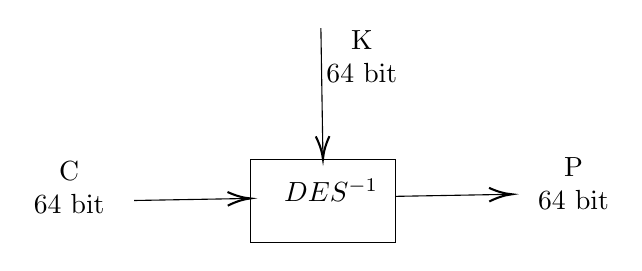
\begin{tikzpicture}[x=0.75pt,y=0.75pt,yscale=-1,xscale=1]
        \draw   (263,99) -- (333,99) -- (333,139) -- (263,139) -- cycle ;
        \draw    (297,35.8) -- (297.97,96.8) ;
        \draw [shift={(298,98.8)}, rotate = 269.09] [color={rgb, 255:red, 0; green, 0; blue, 0 }  ][line width=0.75]    (10.93,-3.29) .. controls (6.95,-1.4) and (3.31,-0.3) .. (0,0) .. controls (3.31,0.3) and (6.95,1.4) .. (10.93,3.29)   ;
        \draw    (207,118.8) -- (261,117.84) ;
        \draw [shift={(263,117.8)}, rotate = 178.98] [color={rgb, 255:red, 0; green, 0; blue, 0 }  ][line width=0.75]    (10.93,-3.29) .. controls (6.95,-1.4) and (3.31,-0.3) .. (0,0) .. controls (3.31,0.3) and (6.95,1.4) .. (10.93,3.29)   ;
        \draw    (333,116.8) -- (387,115.84) ;
        \draw [shift={(389,115.8)}, rotate = 178.98] [color={rgb, 255:red, 0; green, 0; blue, 0 }  ][line width=0.75]    (10.93,-3.29) .. controls (6.95,-1.4) and (3.31,-0.3) .. (0,0) .. controls (3.31,0.3) and (6.95,1.4) .. (10.93,3.29)   ;
        
        \draw (278,107) node [anchor=north west][inner sep=0.75pt]   [align=left] {$DES^{-1}$};
        
        \draw (297,35.8) node [anchor=north west][inner sep=0.75pt]   [align=left] {
        \begin{minipage}[lt]{27.68pt}\setlength\topsep{0pt}
            \begin{center}
            K\\64 bit
            \end{center}
        \end{minipage}};
    
        \draw (156,98.8) node [anchor=north west][inner sep=0.75pt]   [align=left] {
        \begin{minipage}[lt]{27.68pt}\setlength\topsep{0pt}
            \begin{center}
            C\\64 bit
            \end{center}
        \end{minipage}};
        
        \draw (399,96.8) node [anchor=north west][inner sep=0.75pt]   [align=left] {
        \begin{minipage}[lt]{27.68pt}\setlength\topsep{0pt}
            \begin{center}
            P\\64 bit
            \end{center}
        \end{minipage}};
    
    \end{tikzpicture}
\end{center}

The secret key is 64 bits long with every 8th bit (from MSB side) as a parity bit. For Example, 
\begin{center}
    Key: 0110101$\textcolor{red}{0}$ 1101000$\textcolor{red}{1}$ ..... 1101011$\textcolor{red}{1}$
\end{center}
The red coloured bits are parity bits. These are calculated by xoring the 7 bits prior to each parity bit. Now, if there is an odd number of bits altered in the 7 bits, it can be identified using the parity bit. However, parity bits will not help in identifying an alteration in even number of bits.\\
\newline
The first step of DES is to discard these 8 parity bits and get the final secret key of 56 bits. Hence, DES should provide 56 bit security.\\
\newline
In DES, there are 16 rounds, hence, there will be a round function for every round. DES uses the same round function in every round. For each round, there is a round key $K_i$ which is generated by the key scheduling algorithm. It will take secret key as input and generate the round keys $K_1, K_2, ...., K_{16}$. The length of the round keys generated by the key scheduling algorithm is 48 bits.\\

The round function f for DES is defined as follows:
\begin{center}
    $f: \{0,1\}^{32} \times \{0,1\}^{48} \rightarrow \{0,1\}^{32}$
\end{center}
A flowchart for encrpyting a block of message is given below.

\begin{center}
    \tikzset{every picture/.style={line width=0.75pt}} 
    
    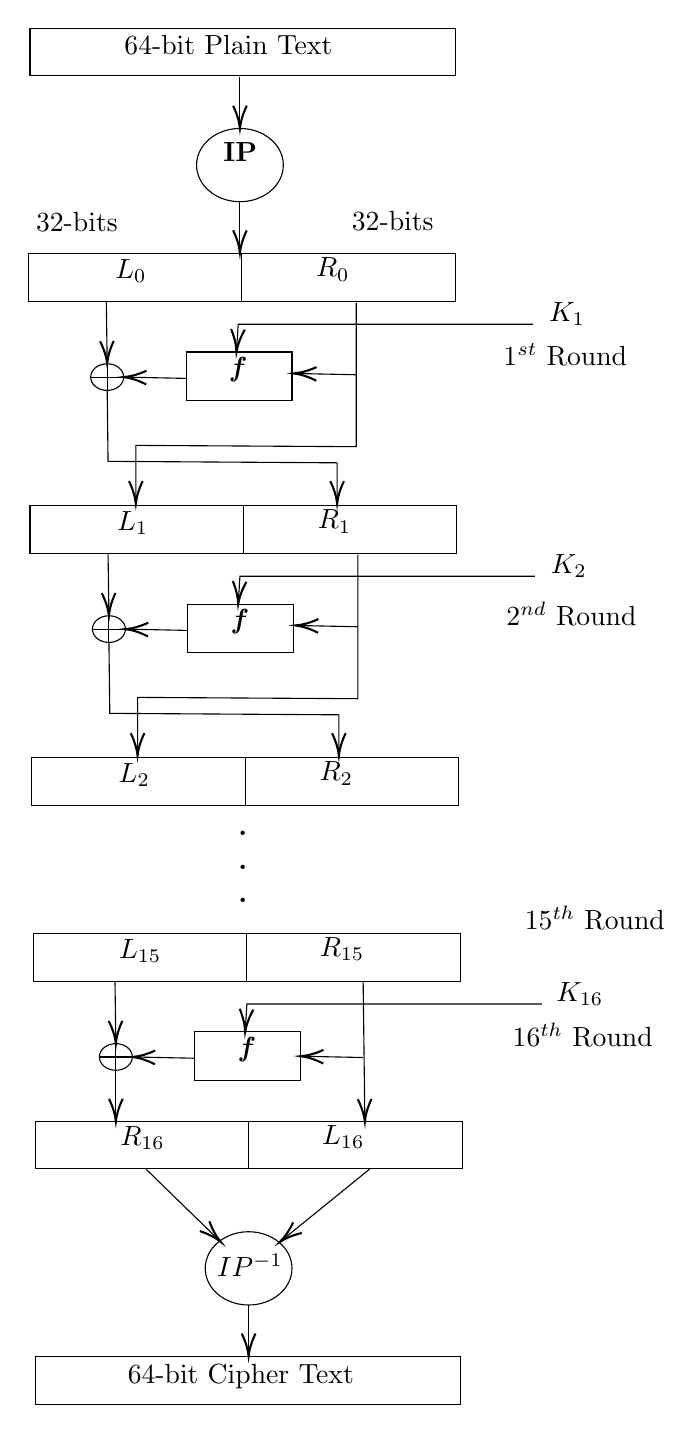
\begin{tikzpicture}[x=0.75pt,y=0.75pt,yscale=-1,xscale=1]
    
    \draw   (192.84,35) -- (397.67,35) -- (397.67,57.87) -- (192.84,57.87) -- cycle ; 
    \draw    (294,58.58) -- (294,81.28) ;
    \draw [shift={(294,83.28)}, rotate = 270] [color={rgb, 255:red, 0; green, 0; blue, 0 }  ][line width=0.75]    (10.93,-3.29) .. controls (6.95,-1.4) and (3.31,-0.3) .. (0,0) .. controls (3.31,0.3) and (6.95,1.4) .. (10.93,3.29)   ; 
    \draw   (273.1,100.93) .. controls (273.1,91.19) and (282.46,83.28) .. (294,83.28) .. controls (305.54,83.28) and (314.9,91.19) .. (314.9,100.93) .. controls (314.9,110.68) and (305.54,118.58) .. (294,118.58) .. controls (282.46,118.58) and (273.1,110.68) .. (273.1,100.93) -- cycle ;
    \draw   (192,143.71) -- (294.84,143.71) -- (294.84,166.58) -- (192,166.58) -- cycle ;
    \draw    (294,118.58) -- (294,141.29) ;
    \draw [shift={(294,143.29)}, rotate = 270] [color={rgb, 255:red, 0; green, 0; blue, 0 }  ][line width=0.75]    (10.93,-3.29) .. controls (6.95,-1.4) and (3.31,-0.3) .. (0,0) .. controls (3.31,0.3) and (6.95,1.4) .. (10.93,3.29)   ;
    \draw   (294.84,143.71) -- (397.67,143.71) -- (397.67,166.58) -- (294.84,166.58) -- cycle ;
    \draw   (268.08,191.01) -- (319.08,191.01) -- (319.08,214.44) -- (268.08,214.44) -- cycle ; 
    \draw   (222.1,203.08) .. controls (222.1,199.53) and (225.65,196.66) .. (230.04,196.66) .. controls (234.43,196.66) and (237.98,199.53) .. (237.98,203.08) .. controls (237.98,206.63) and (234.43,209.5) .. (230.04,209.5) .. controls (225.65,209.5) and (222.1,206.63) .. (222.1,203.08) -- cycle ; \draw   (222.1,203.08) -- (237.98,203.08) ; \draw   (230.04,196.66) -- (230.04,209.5) ;
    \draw    (350.02,167.29) -- (350.02,236.61) -- (253.87,236.04) -- (243.84,235.98) -- (243.84,262.14) ;
    \draw [shift={(243.84,264.14)}, rotate = 270] [color={rgb, 255:red, 0; green, 0; blue, 0 }  ][line width=0.75]    (10.93,-3.29) .. controls (6.95,-1.4) and (3.31,-0.3) .. (0,0) .. controls (3.31,0.3) and (6.95,1.4) .. (10.93,3.29)   ;
    \draw   (192.84,265.13) -- (295.67,265.13) -- (295.67,288) -- (192.84,288) -- cycle ;
    \draw   (295.67,265.13) -- (398.51,265.13) -- (398.51,288) -- (295.67,288) -- cycle ;
    \draw    (350.02,201.95) -- (321.92,201.36) ;
    \draw [shift={(319.92,201.31)}, rotate = 1.21] [color={rgb, 255:red, 0; green, 0; blue, 0 }  ][line width=0.75]    (10.93,-3.29) .. controls (6.95,-1.4) and (3.31,-0.3) .. (0,0) .. controls (3.31,0.3) and (6.95,1.4) .. (10.93,3.29)   ;
    \draw    (268.08,203.71) -- (239.98,203.12) ;
    \draw [shift={(237.98,203.08)}, rotate = 1.21] [color={rgb, 255:red, 0; green, 0; blue, 0 }  ][line width=0.75]    (10.93,-3.29) .. controls (6.95,-1.4) and (3.31,-0.3) .. (0,0) .. controls (3.31,0.3) and (6.95,1.4) .. (10.93,3.29)   ;
    \draw    (229.62,166.58) -- (230.01,194.66) ;
    \draw [shift={(230.04,196.66)}, rotate = 269.2] [color={rgb, 255:red, 0; green, 0; blue, 0 }  ][line width=0.75]    (10.93,-3.29) .. controls (6.95,-1.4) and (3.31,-0.3) .. (0,0) .. controls (3.31,0.3) and (6.95,1.4) .. (10.93,3.29)   ; 
    \draw    (230.04,209.5) -- (230.46,243.67) -- (340.82,244.38) -- (340.82,262.14) ;
    \draw [shift={(340.82,264.14)}, rotate = 270] [color={rgb, 255:red, 0; green, 0; blue, 0 }  ][line width=0.75]    (10.93,-3.29) .. controls (6.95,-1.4) and (3.31,-0.3) .. (0,0) .. controls (3.31,0.3) and (6.95,1.4) .. (10.93,3.29)   ;
    \draw    (435.3,177.6) -- (293.16,177.6) -- (292.45,189.01) ;
    \draw [shift={(292.33,191.01)}, rotate = 273.57] [color={rgb, 255:red, 0; green, 0; blue, 0 }  ][line width=0.75]    (10.93,-3.29) .. controls (6.95,-1.4) and (3.31,-0.3) .. (0,0) .. controls (3.31,0.3) and (6.95,1.4) .. (10.93,3.29)   ;
    \draw   (268.92,312.43) -- (319.92,312.43) -- (319.92,335.86) -- (268.92,335.86) -- cycle ; 
    \draw   (222.93,324.5) .. controls (222.93,320.95) and (226.49,318.07) .. (230.88,318.07) .. controls (235.26,318.07) and (238.82,320.95) .. (238.82,324.5) .. controls (238.82,328.05) and (235.26,330.92) .. (230.88,330.92) .. controls (226.49,330.92) and (222.93,328.05) .. (222.93,324.5) -- cycle ; \draw   (222.93,324.5) -- (238.82,324.5) ; \draw   (230.88,318.07) -- (230.88,330.92) ;
    \draw    (350.85,288.71) -- (350.85,358.03) -- (254.71,357.46) -- (244.67,357.4) -- (244.67,383.56) ;
    \draw [shift={(244.67,385.56)}, rotate = 270] [color={rgb, 255:red, 0; green, 0; blue, 0 }  ][line width=0.75]    (10.93,-3.29) .. controls (6.95,-1.4) and (3.31,-0.3) .. (0,0) .. controls (3.31,0.3) and (6.95,1.4) .. (10.93,3.29)   ; 
    \draw   (193.67,386.55) -- (296.51,386.55) -- (296.51,409.42) -- (193.67,409.42) -- cycle ;
    \draw   (296.51,386.55) -- (399.35,386.55) -- (399.35,409.42) -- (296.51,409.42) -- cycle ;
    \draw    (350.85,323.37) -- (322.75,322.78) ;
    \draw [shift={(320.76,322.73)}, rotate = 1.21] [color={rgb, 255:red, 0; green, 0; blue, 0 }  ][line width=0.75]    (10.93,-3.29) .. controls (6.95,-1.4) and (3.31,-0.3) .. (0,0) .. controls (3.31,0.3) and (6.95,1.4) .. (10.93,3.29)   ; 
    \draw    (268.92,325.13) -- (240.82,324.54) ;
    \draw [shift={(238.82,324.5)}, rotate = 1.21] [color={rgb, 255:red, 0; green, 0; blue, 0 }  ][line width=0.75]    (10.93,-3.29) .. controls (6.95,-1.4) and (3.31,-0.3) .. (0,0) .. controls (3.31,0.3) and (6.95,1.4) .. (10.93,3.29)   ;
    \draw    (230.46,288) -- (230.85,316.07) ;
    \draw [shift={(230.88,318.07)}, rotate = 269.2] [color={rgb, 255:red, 0; green, 0; blue, 0 }  ][line width=0.75]    (10.93,-3.29) .. controls (6.95,-1.4) and (3.31,-0.3) .. (0,0) .. controls (3.31,0.3) and (6.95,1.4) .. (10.93,3.29)   ;
    \draw    (230.88,330.92) -- (231.3,365.09) -- (341.66,365.79) -- (341.66,383.56) ;
    \draw [shift={(341.66,385.56)}, rotate = 270] [color={rgb, 255:red, 0; green, 0; blue, 0 }  ][line width=0.75]    (10.93,-3.29) .. controls (6.95,-1.4) and (3.31,-0.3) .. (0,0) .. controls (3.31,0.3) and (6.95,1.4) .. (10.93,3.29)   ;
    \draw    (436.13,299.01) -- (294,299.01) -- (293.29,310.43) ;
    \draw [shift={(293.16,312.43)}, rotate = 273.57] [color={rgb, 255:red, 0; green, 0; blue, 0 }  ][line width=0.75]    (10.93,-3.29) .. controls (6.95,-1.4) and (3.31,-0.3) .. (0,0) .. controls (3.31,0.3) and (6.95,1.4) .. (10.93,3.29)   ;
    \draw   (194.51,471.26) -- (297.35,471.26) -- (297.35,494.13) -- (194.51,494.13) -- cycle ; 
    \draw   (297.35,471.26) -- (400.18,471.26) -- (400.18,494.13) -- (297.35,494.13) -- cycle ;
    \draw   (272.26,518.56) -- (323.26,518.56) -- (323.26,541.99) -- (272.26,541.99) -- cycle ;
    \draw   (226.28,530.63) .. controls (226.28,527.08) and (229.84,524.2) .. (234.22,524.2) .. controls (238.61,524.2) and (242.16,527.08) .. (242.16,530.63) .. controls (242.16,534.17) and (238.61,537.05) .. (234.22,537.05) .. controls (229.84,537.05) and (226.28,534.17) .. (226.28,530.63) -- cycle ; \draw   (226.28,530.63) -- (242.16,530.63) ; \draw   (234.22,524.2) -- (234.22,537.05) ;
    \draw    (233.8,494.13) -- (234.19,522.2) ;
    \draw [shift={(234.22,524.2)}, rotate = 269.2] [color={rgb, 255:red, 0; green, 0; blue, 0 }  ][line width=0.75]    (10.93,-3.29) .. controls (6.95,-1.4) and (3.31,-0.3) .. (0,0) .. controls (3.31,0.3) and (6.95,1.4) .. (10.93,3.29)   ;
    \draw    (439.48,505.14) -- (297.35,505.14) -- (296.63,516.56) ;
    \draw [shift={(296.51,518.56)}, rotate = 273.57] [color={rgb, 255:red, 0; green, 0; blue, 0 }  ][line width=0.75]    (10.93,-3.29) .. controls (6.95,-1.4) and (3.31,-0.3) .. (0,0) .. controls (3.31,0.3) and (6.95,1.4) .. (10.93,3.29)   ;
    \draw   (195.34,561.62) -- (298.18,561.62) -- (298.18,584.49) -- (195.34,584.49) -- cycle ;
    \draw   (298.18,561.62) -- (401.02,561.62) -- (401.02,584.49) -- (298.18,584.49) -- cycle ;
    \draw    (353.36,530.91) -- (325.26,530.32) ;
    \draw [shift={(323.26,530.27)}, rotate = 1.21] [color={rgb, 255:red, 0; green, 0; blue, 0 }  ][line width=0.75]    (10.93,-3.29) .. controls (6.95,-1.4) and (3.31,-0.3) .. (0,0) .. controls (3.31,0.3) and (6.95,1.4) .. (10.93,3.29)   ;
    \draw    (353.36,494.13) -- (354.17,559.9) ;
    \draw [shift={(354.2,561.9)}, rotate = 269.29] [color={rgb, 255:red, 0; green, 0; blue, 0 }  ][line width=0.75]    (10.93,-3.29) .. controls (6.95,-1.4) and (3.31,-0.3) .. (0,0) .. controls (3.31,0.3) and (6.95,1.4) .. (10.93,3.29)   ;
    \draw    (234.22,537.05) -- (234.22,559.76) ;
    \draw [shift={(234.22,561.76)}, rotate = 270] [color={rgb, 255:red, 0; green, 0; blue, 0 }  ][line width=0.75]    (10.93,-3.29) .. controls (6.95,-1.4) and (3.31,-0.3) .. (0,0) .. controls (3.31,0.3) and (6.95,1.4) .. (10.93,3.29)   ;
    \draw   (277.28,632.49) .. controls (277.28,622.74) and (286.64,614.84) .. (298.18,614.84) .. controls (309.73,614.84) and (319.08,622.74) .. (319.08,632.49) .. controls (319.08,642.24) and (309.73,650.14) .. (298.18,650.14) .. controls (286.64,650.14) and (277.28,642.24) .. (277.28,632.49) -- cycle ; 
    \draw    (248.85,584.77) -- (283.37,618.39) ;
    \draw [shift={(284.8,619.78)}, rotate = 224.24] [color={rgb, 255:red, 0; green, 0; blue, 0 }  ][line width=0.75]    (10.93,-3.29) .. controls (6.95,-1.4) and (3.31,-0.3) .. (0,0) .. controls (3.31,0.3) and (6.95,1.4) .. (10.93,3.29)   ;
    \draw    (356.71,584.49) -- (314.78,618.52) ;
    \draw [shift={(313.23,619.78)}, rotate = 320.93] [color={rgb, 255:red, 0; green, 0; blue, 0 }  ][line width=0.75]    (10.93,-3.29) .. controls (6.95,-1.4) and (3.31,-0.3) .. (0,0) .. controls (3.31,0.3) and (6.95,1.4) .. (10.93,3.29)   ; 
    \draw    (298.18,650.14) -- (298.18,672.85) ;
    \draw [shift={(298.18,674.85)}, rotate = 270] [color={rgb, 255:red, 0; green, 0; blue, 0 }  ][line width=0.75]    (10.93,-3.29) .. controls (6.95,-1.4) and (3.31,-0.3) .. (0,0) .. controls (3.31,0.3) and (6.95,1.4) .. (10.93,3.29)   ;
    \draw   (195.34,675.13) -- (400.18,675.13) -- (400.18,698) -- (195.34,698) -- cycle ;
    \draw    (272.26,531.26) -- (244.16,530.67) ;
    \draw [shift={(242.16,530.63)}, rotate = 1.21] [color={rgb, 255:red, 0; green, 0; blue, 0 }  ][line width=0.75]    (10.93,-3.29) .. controls (6.95,-1.4) and (3.31,-0.3) .. (0,0) .. controls (3.31,0.3) and (6.95,1.4) .. (10.93,3.29)   ;
    
    \draw (237.08,37.29) node [anchor=north west][inner sep=0.75pt]   [align=left] {64-bit Plain Text};
    \draw (284.76,88.65) node [anchor=north west][inner sep=0.75pt]   [align=left] {\textbf{IP}};
    \draw (232.67,145.12) node [anchor=north west][inner sep=0.75pt]   [align=left] {$L_0$};
    \draw (329.49,144.42) node [anchor=north west][inner sep=0.75pt]   [align=left] {$R_0$};
    \draw (194.51,122.53) node [anchor=north west][inner sep=0.75pt]   [align=left] {32-bits};
    \draw (346.67,121.83) node [anchor=north west][inner sep=0.75pt]   [align=left] {32-bits};
    \draw (288.51,192.42) node [anchor=north west][inner sep=0.75pt]   [align=left] {\textbf{\textit{f}}};
    \draw (233.51,266.54) node [anchor=north west][inner sep=0.75pt]   [align=left] {$L_1$};
    \draw (330.33,265.84) node [anchor=north west][inner sep=0.75pt]   [align=left] {$R_1$};
    \draw (441.71,165.88) node [anchor=north west][inner sep=0.75pt]   [align=left] {$K_1$};
    \draw (419.71,185.7) node [anchor=north west][inner sep=0.75pt]   [align=left] {$1^{st}$ Round};
    \draw (289.35,313.84) node [anchor=north west][inner sep=0.75pt]   [align=left] {\textbf{\textit{f}}};
    \draw (234.34,387.96) node [anchor=north west][inner sep=0.75pt]   [align=left] {$L_2$};
    \draw (331.17,387.25) node [anchor=north west][inner sep=0.75pt]   [align=left] {$R_2$};
    \draw (442.54,287.3) node [anchor=north west][inner sep=0.75pt]   [align=left] {$K_2$};
    \draw (421.13,310.12) node [anchor=north west][inner sep=0.75pt]   [align=left] {$2^{nd}$ Round};
    \draw (234.53,472.67) node [anchor=north west][inner sep=0.75pt]   [align=left] {$L_{15}$};
    \draw (331.26,471.97) node [anchor=north west][inner sep=0.75pt]   [align=left] {$R_{15}$};
    \draw (430,456.72) node [anchor=north west][inner sep=0.75pt]   [align=left] {$15^{th}$ Round};
    \draw (292.69,519.97) node [anchor=north west][inner sep=0.75pt]   [align=left] {\textbf{\textit{f}}};
    \draw (445.23,493.43) node [anchor=north west][inner sep=0.75pt]   [align=left] {$K_{16}$};
    \draw (424.15,513.25) node [anchor=north west][inner sep=0.75pt]   [align=left] {$16^{th}$ Round};
    \draw (235.12,563.03) node [anchor=north west][inner sep=0.75pt]   [align=left] {$R_{16}$};
    \draw (332.35,562.32) node [anchor=north west][inner sep=0.75pt]   [align=left] {$L_{16}$};
    \draw (281.79,624.21) node [anchor=north west][inner sep=0.75pt]   [align=left] {\textbf{$IP^{-1}$}};
    \draw (238.69,677.42) node [anchor=north west][inner sep=0.75pt]   [align=left] {64-bit Cipher Text};
    \draw (292,420.8) node [anchor=north west][inner sep=0.75pt]   [align=left] {\textbf{.}\\\textbf{.}\\\textbf{.}\\};
\end{tikzpicture}
\end{center}
In the flowchart above, IP is the initial permutation and it will permute the message bits. Similar to Feistel Network, for each round $L_{i+1}$ and $R_{i+1}$ will be:
\begin{center}
    $L_{i+1} = R_i$\\
    $R_{i+1} = L_i \oplus f(R_i, K_{i+1})$
\end{center}
where $i \in \{0, 1,..., 15\}$. In the last round, i.e. $16^{th}$ round, the position of $L_{16}$ and $R_{16}$ are swapped. After this round, the inverse of Initial Permutation (IP) is applied to the 64-bits and we get the cipher text.\\
\newline
We need to address the following now:
\begin{itemize}
    \item Initial Permutation and its inverse
    \item The round function $f$
    \item How are the round keys $K_1, K_2, ...., K_{16}$ generated.
\end{itemize}

\subsection{Initial Permutation of DES}
It is a bijection from 64-bit to 64-bit. The 64-bits of the message are permuted and then the rounds are applied to the permuted message. Initial Permutation is defined as:
\begin{center}
IP =  
    $\begin{bmatrix}
    58 & 50 & 42 & 34 & 26 & 18 & 10 & 2\\
    60 & 52 & 44 & 36 & 28 & 20 & 12 & 4\\
    62 & 54 & 46 & 38 & 30 & 22 & 14 & 6\\
    64 & 56 & 48 & 40 & 32 & 24 & 16 & 8\\
    57 & 49 & 41 & 33 & 25 & 17 & 9 & 1\\
    59 & 51 & 43 & 35 & 27 & 19 & 11 & 3\\
    61 & 53 & 45 & 37 & 29 & 21 & 13 & 5\\
    63 & 55 & 47 & 39 & 31 & 23 & 15 & 7\\
    \end{bmatrix}$
\end{center}
It can be interpreted as follows:
\begin{center}
    $IP(m_1m_2...m_7m_8m_9....m_{64}) = m_{58}m_{50}...m_{10}m_2m_{60}....m_7 $
\end{center}
Using IP we can easily compute its inverse. The inverse of IP is provided in the \hyperref[appendix]{Appendix}


\subsection{Round Function of DES}
\begin{center}
    $f: \{0,1\}^{32} \times \{0,1\}^{48} \rightarrow \{0,1\}^{32}$\\
    $f(R_i, K_i) = X_i$\\
    where $R_i$ is 32-bit, $K_i$ is 48-bit and $X_i$ is 32-bit.
\end{center}
The round function for DES is defined as:
\begin{center}
    $f(R_i, K_i) = P(S(E(R_i) \oplus K_i))$\\
\end{center}
\begin{center}
    Expansion Function E : $\{0, 1\}^{32} \rightarrow \{0, 1\}^{48}$\\
    Substitution Box S: $\{0, 1\}^{48} \rightarrow \{0, 1\}^{32}$\\
    Permutation Box P: $\{0, 1\}^{32} \rightarrow \{0, 1\}^{32}$\\
\end{center}
Hence,
\begin{center}
    length of $R_i$ = 32-bits\\
    length of $E(R_i)$ = 48-bits = length of $K_i$\\
    length of $E(R_i) \oplus K_i$ = 48-bits\\
    length of $S(E(R_i) \oplus K_i)$ = 32-bits\\
    length of $P(S(E(R_i) \oplus K_i))$ = 32-bits
\end{center}

\subsubsection{Expansion Function}
\begin{center}
    $E: \{0, 1\}^{32} \rightarrow \{0, 1\}^{48}$\\    
\end{center}

The expansion function for DES is given below:
\begin{center}
    $ E = 
    \begin{bmatrix}
        32 & 1 & 2 & 3 & 4 & 5\\
        4 & 5 & 6 & 7 & 8 & 9\\
        8 & 9 & 10 & 11 & 12 & 13\\
        12 & 13 & 14 & 15 & 16 & 17\\
        16 & 17 & 18 & 19 & 20 & 21\\
        20 & 21 & 22 & 23 & 24 & 25\\
        24 & 25 & 26 & 27 & 28 & 29\\
        28 & 29 & 30 & 31 & 32 & 1\\
    \end{bmatrix}$
\end{center}
The bits are repeated for expanding 32-bits to 48-bits.

\begin{center}
    $E(x_1x_2....x_{32}) = (x_{32}x_1x_2x_3x_4x_5x_4x_5....x_{32}x_1)$
\end{center}

\subsubsection{Substitution Box}
\begin{center}
    $S: \{0, 1\}^{48} \rightarrow \{0, 1\}^{32}$\\
    $S(X) = Y$,  where X is 48 and Y is 32 bit long
\end{center}
Dividing X into 8 blocks each of length 6-bits.
\begin{center}
    $X = B_1B_2B_3B_4B_5B_6B_7B_8$\\
\end{center}
Corresponding to each $B_i$ there is a substitution box $S_i$ where $i \in \{1,2,..,8\}$.
\begin{center}
    $S_i: \{0, 1\}^6 \rightarrow \{0, 1\}^4  \forall i \in \{1,2,..,8\}$\\
    $S_i(B_i) = C_i$\\
    $\therefore S(X) = (S_1(B_1), S_2(B_2), S_3(B_3), S_4(B_4), S_5(B_5), S_6(B_6), S_7(B_7), S_8(B_8))$ 
\end{center}
Therefore, length of S(X) is 32 bits. Now, let's see how to compute the output $C_i$ given $S_i$ and $B_i$. There is a $4 \times 16$ table corresponding to each $S_i$ for DES. These tables are provided in the \hyperref[appendix]{Appendix}.\\
\begin{center}
    $ S_i = 
    \begin{bmatrix}
        a_{0,0} & \dots & a_{0,15}\\
        \vdots & \ddots & \vdots\\
        a_{3,0} & \dots & a_{3,15}\\
    \end{bmatrix}$ 
    where $a_{i,j} \in \{0, 1,...15\}$
\end{center}

Lets see how we have to look into these tables. Consider the binary representation of $B_i$.
\begin{center}
    $B_i = b_1b_2b_3b_4b_5b_6$ where $b_i \in \{0, 1\}$
\end{center}
Now, consider the MSB and LSB of $B_i$, i.e $b_1$ and $b_6$. The decimal value of the binary number $b_1b_6$ will be:
\begin{center}
    $r = 2 \cdot b_1 + b_6$\\
    $\therefore r \in \{0, 1, 2, 3\}$ 
\end{center}
$r$ is called the row number. Now, consider the rest of the bits of $B_i$, i.e. $b_2b_3b_4b_5$. The decimal value of $b_2b_3b_4b_5$ (denoted by c) will be an integer in $0 \leq c \leq 15$. This c is called as the column number. The value of $S_i(B_i)$ is the entry in $S_i$ table in row $r$ and column $c$.
\begin{center}
    $S_i(B_i) = a_{r,c}$
\end{center}

\subsubsection{Permutation Box}
\begin{center}
    $P: \{0, 1\}^{32} \rightarrow \{0, 1\}^{32}$\\
\end{center}
It is also defined by a table. The table is given below:
\begin{center}
    $ P = 
    \begin{bmatrix}
        16 & 7 & 20 & 21\\
        29 & 12 & 28 & 17\\
        1 & 15 & 23 & 26\\
        5 & 18 & 31 & 10\\
        2 & 8 & 24 & 14\\
        32 & 27 & 3 & 9\\
        19 & 13 & 30 & 6\\
        22 & 11 & 4 & 25\\
    \end{bmatrix}$\\
\end{center}
\begin{center}
    $P(x_1x_2...x_{32}) = x_{16}x_7x_{20}x_{21}x_{29}...x_{25}$
\end{center}

\subsection{Key Scheduling Algorithm of DES}
The Key Scheduling Algorithm generates round keys for each of the 16 rounds of DES. It takes the 64-bit secret key as input and produces 16 round keys, each of 48-bits.\\
The steps of the algorithm are given below:
\begin{itemize}
    \item Define $v_i, 1 \leq i \leq 16$, where $v_i = 1$ if $i \in \{1, 2, 9, 16\}$, else $v_i = 2$. 
    \item Discard 8 parity check bits from K. The 56 bit key is $\Tilde{K}$.
    \item $T = PC1(\Tilde{K})$, where PC1 is a permuation defined as:
    \begin{center}
        $PC1: \{0, 1\}^{56} \rightarrow \{0, 1\}^{56}$\\
    \end{center}

    \item $(C_0, D_0) = T$, where $C_0$ is most significant 28 bits of T and $D_0$ is least significant 28 bits of T.

    \item for $i = 1$ to 16:
    \begin{center}
        $C_i = (C_{i-1} \hookleftarrow v_i)$\\
        $D_i = (D_{i-1} \hookleftarrow v_i)$\\
    \end{center}
    $\hookleftarrow$ is left circular shift. For Example: $x_1x_2...x_{25} \hookleftarrow 2 = x_3x_4....x_{25}x_1x_2$.
    \begin{center}
        $K_i = PC2(C_i, D_i)$\\
    \end{center}
    where, PC2 is a substitution defined as:
    \begin{center}
        $PC2: \{0, 1\}^{56} \rightarrow \{0, 1\}^{48}$\\
    \end{center}

    \item Round Keys = $\{K_1, K_2,...., K_{16}\}$
\end{itemize}

\subsubsection{PC1}

\begin{center}
    $PC1: \{0, 1\}^{56} \rightarrow \{0, 1\}^{56}$\\
\end{center}

\begin{center}
PC1 =  
    $\begin{bmatrix}
    57 & 49 & 41 & 33 & 25 & 17 & 9\\
    1 & 58 & 50 & 42 & 34 & 26 & 18\\
    10 & 2 & 59 & 51 & 43 & 35 & 27\\
    19 & 11 & 3 & 60 & 52 & 44 & 36\\
    63 & 55 & 47 & 39 & 31 & 23 & 15\\
    7 & 62 & 54 & 46 & 38 & 30 & 22\\
    14 & 6 & 61 & 53 & 45 & 37 & 29\\
    21 & 13 & 5 & 28 & 20 & 12 & 4\\
    \end{bmatrix}$
\end{center}
 Input to PC1 is the 56-bit key $\Tilde{K}$ and the output is $T$.
 \begin{center}
     $T = PC1(K_1K_2...K_7K_9K_{10}....K_{63}) = K_{57}K_{49}....K_{12}K_4$
 \end{center}
 The 28 MSB of T is $C_i$ while 28 LSB is $D_i$.

 \subsubsection{PC2}
\begin{center}
    $PC2: \{0, 1\}^{56} \rightarrow \{0, 1\}^{48}$\\
\end{center}
\begin{center}
    PC2 = 
    $\begin{bmatrix}
        14 & 17 & 11 & 24 & 1 & 5\\
        3 & 28 & 15 & 6 & 21 & 10\\
        23 & 19 & 12 & 4 & 26 & 8\\
        16 & 7 & 27 & 20 & 13 & 2\\
        41 & 52 & 31 & 37 & 47 & 55\\
        30 & 40 & 51 & 45 & 33 & 48\\
        44 & 49 & 39 & 56 & 34 & 53\\
        46 & 42 & 50 & 36 & 29 & 32\\
    \end{bmatrix}$
\end{center}
\begin{center}
    $K_i = PC2(C_i, D_i) = PC2(x_1x_2...x_{56}) = x_{14}x_{17}...x_{32}$
\end{center}

\section{Complementation Property of DES}
Let us consider the Feistel Network structure agian.
\begin{center}
    \tikzset{every picture/.style={line width=0.75pt}}       
    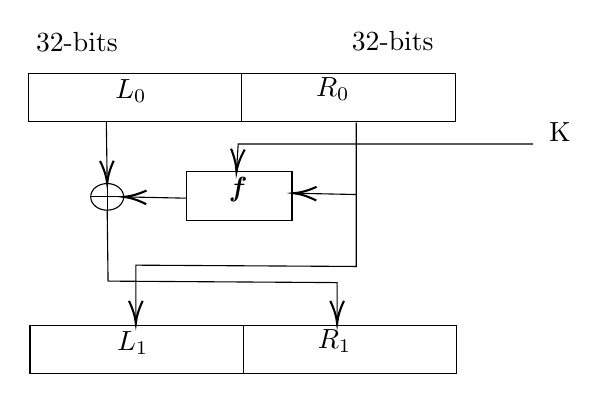
\begin{tikzpicture}[x=0.75pt,y=0.75pt,yscale=-1,xscale=1]
    
    \draw   (192,143.71) -- (294.84,143.71) -- (294.84,166.58) -- (192,166.58) -- cycle ;
    \draw   (294.84,143.71) -- (397.67,143.71) -- (397.67,166.58) -- (294.84,166.58) -- cycle ;
    \draw   (268.08,191.01) -- (319.08,191.01) -- (319.08,214.44) -- (268.08,214.44) -- cycle ;
    \draw   (222.1,203.08) .. controls (222.1,199.53) and (225.65,196.66) .. (230.04,196.66) .. controls (234.43,196.66) and (237.98,199.53) .. (237.98,203.08) .. controls (237.98,206.63) and (234.43,209.5) .. (230.04,209.5) .. controls (225.65,209.5) and (222.1,206.63) .. (222.1,203.08) -- cycle ; \draw   (222.1,203.08) -- (237.98,203.08) ; \draw   (230.04,196.66) -- (230.04,209.5) ;
    \draw    (350.02,167.29) -- (350.02,236.61) -- (253.87,236.04) -- (243.84,235.98) -- (243.84,262.14) ;
    \draw [shift={(243.84,264.14)}, rotate = 270] [color={rgb, 255:red, 0; green, 0; blue, 0 }  ][line width=0.75]    (10.93,-3.29) .. controls (6.95,-1.4) and (3.31,-0.3) .. (0,0) .. controls (3.31,0.3) and (6.95,1.4) .. (10.93,3.29)   ;
    \draw   (192.84,265.13) -- (295.67,265.13) -- (295.67,288) -- (192.84,288) -- cycle ;
    \draw   (295.67,265.13) -- (398.51,265.13) -- (398.51,288) -- (295.67,288) -- cycle ;
    \draw    (350.02,201.95) -- (321.92,201.36) ;
    \draw [shift={(319.92,201.31)}, rotate = 1.21] [color={rgb, 255:red, 0; green, 0; blue, 0 }  ][line width=0.75]    (10.93,-3.29) .. controls (6.95,-1.4) and (3.31,-0.3) .. (0,0) .. controls (3.31,0.3) and (6.95,1.4) .. (10.93,3.29)   ;
    \draw    (268.08,203.71) -- (239.98,203.12) ;
    \draw [shift={(237.98,203.08)}, rotate = 1.21] [color={rgb, 255:red, 0; green, 0; blue, 0 }  ][line width=0.75]    (10.93,-3.29) .. controls (6.95,-1.4) and (3.31,-0.3) .. (0,0) .. controls (3.31,0.3) and (6.95,1.4) .. (10.93,3.29)   ;
    \draw    (229.62,166.58) -- (230.01,194.66) ;
    \draw [shift={(230.04,196.66)}, rotate = 269.2] [color={rgb, 255:red, 0; green, 0; blue, 0 }  ][line width=0.75]    (10.93,-3.29) .. controls (6.95,-1.4) and (3.31,-0.3) .. (0,0) .. controls (3.31,0.3) and (6.95,1.4) .. (10.93,3.29)   ;
    \draw    (230.04,209.5) -- (230.46,243.67) -- (340.82,244.38) -- (340.82,262.14) ;
    \draw [shift={(340.82,264.14)}, rotate = 270] [color={rgb, 255:red, 0; green, 0; blue, 0 }  ][line width=0.75]    (10.93,-3.29) .. controls (6.95,-1.4) and (3.31,-0.3) .. (0,0) .. controls (3.31,0.3) and (6.95,1.4) .. (10.93,3.29)   ;
    \draw    (435.3,177.6) -- (293.16,177.6) -- (292.45,189.01) ;
    \draw [shift={(292.33,191.01)}, rotate = 273.57] [color={rgb, 255:red, 0; green, 0; blue, 0 }  ][line width=0.75]    (10.93,-3.29) .. controls (6.95,-1.4) and (3.31,-0.3) .. (0,0) .. controls (3.31,0.3) and (6.95,1.4) .. (10.93,3.29)   ;
    
    \draw (232.67,145.12) node [anchor=north west][inner sep=0.75pt]   [align=left] {$L_0$};
    \draw (329.49,144.42) node [anchor=north west][inner sep=0.75pt]   [align=left] {$R_0$};
    \draw (194.51,122.53) node [anchor=north west][inner sep=0.75pt]   [align=left] {32-bits};
    \draw (346.67,121.83) node [anchor=north west][inner sep=0.75pt]   [align=left] {32-bits};
    \draw (288.51,192.42) node [anchor=north west][inner sep=0.75pt]   [align=left] {\textbf{\textit{f}}};
    \draw (233.51,266.54) node [anchor=north west][inner sep=0.75pt]   [align=left] {$L_1$};
    \draw (330.33,265.84) node [anchor=north west][inner sep=0.75pt]   [align=left] {$R_1$};
    \draw (441.71,165.88) node [anchor=north west][inner sep=0.75pt]   [align=left] {K};
    
    \end{tikzpicture}
\end{center}
Let us call this structure FN and it takes the message and key as input and generates the cipher text. The following are now known to us:
\begin{center}
    $M = L_0 || R_0$ (the message)\\
    $f = P(S(E(R_0) \oplus K))$ \\
    $C = L_1 || R_1$ (the cipher text)
\end{center}
Now, consider the following two equations:
\begin{center}
    $FN(M, K) = C_1$\\
    $FN(\overline{M}, \overline{K}) = C_2$\\
\end{center}
where $\overline{X}$ denotes bitwise complement of $X$. That is, if:
\begin{center}
    $X = x_1x_2.....x_n$\\
    $\overline{X} = (1\oplus x_1)(1 \oplus x_2)....(1 \oplus x_n)$
\end{center}
Let us try to find a relation between $C_1$ and $C_2$. Clearly,
\begin{center}
    $L_{1M} = R_{0M}$ and $L_{1\overline{M}} = R_{0\overline{M}}$\\
\end{center}
$R_{0M}$ and $R_{0\overline{M}}$ are bit-wise complementary to each other $(\because M$ and $\overline{M}$ are complementary). Therefore, $L_{1M}$ and $L_{1\overline{M}}$ are complementary.\\
\newline
Now, let's try to find the relation between $f(M, K)$ and $f(\overline{M}, \overline{K})$. Let's say $R_0 = x_1x_2....x_{32}$. Therefore,
\begin{center}
    $\overline{R_0} = \overline{x_1} \overline{x_2}...\overline{x_{32}}$\\
    $\implies E(\overline{R_0}) = \overline{x_{32}}\overline{x_1}...\overline{x_1}$\\
    $\implies E(\overline{R_0}) = \overline{x_{32}x_{1}...x_1}$\\
    $\implies E(\overline{R_0}) = \overline{E(R_0)}$
\end{center}
Now, from the definition of round function $f$:
\begin{center}
    $f(\overline{M}, \overline{K}) = P(S(E({R_{0\overline{M}}}) \oplus \overline{K}))$\\
    \vspace{2mm}
    $f(\overline{M}, \overline{K}) = P(S(E({\overline{R_{0M}}}) \oplus \overline{K}))$\\
    \hfill (because $M$ and $\overline{M}$ are complementary)\\
    $f(\overline{M}, \overline{K}) = P(S(\overline{E(R_{0M})} \oplus \overline{K}))$ (proved above)\\
    \vspace{2mm}
    $f(\overline{M}, \overline{K}) = P(S({E(R_{0M})} \oplus {K}))$\\
    \hfill $(\because A \oplus B = \overline{A} \oplus \overline{B})$\\
    $f(\overline{M}, \overline{K}) = f(M, K)$\\
\end{center}
Since, S and P are substituion and permuation respectively, they will generate same output if given the same input. Now, 
\begin{center}
    $R_{1M} = L_{0M} \oplus f(M, K)$ and $R_{1\overline{M}} = L_{0\overline{M}} \oplus f(\overline{M}, \overline{K})$\\
    \vspace{2mm}
    $\implies R_{1M} = L_{0M} \oplus f(M, K)$ and $R_{1\overline{M}} = L_{0\overline{M}} \oplus f(M,K)$\\
\end{center}
Since, $L_{0M}$ and $L_{0\overline{M}}$ are complementary, $R_{1M}$ and $R_{1\overline{M}}$ should also be complementary. Since, 
\begin{center}
    $C_2 = L_{1\overline{M}} || R_{1\overline{M}}$\\
    \vspace{2mm}
    $C_2 = \overline{L_{1M}} || \overline{R_{1M}}$\\
    \vspace{2mm}
    $C_2 = \overline{L_{1M} || R_{1M}}$\\
    \vspace{2mm}
    $C_2 = \overline{C_1}$
\end{center}
Hence, for Feistel Networks, the outputs will be complement to each other, if the messages and keys are complementary to each other.\\
\newline
The key scheduling algorithm for DES performs a permutation, a left circular shift and then a substitution. Since, these operations are exactly similar for each input, therefore, if two complementary inputs are given to the key scheduling algorithm:
\begin{itemize}
    \item Left Circular Shift will generate complemented outputs.
    \item PC1 will generate complemented outputs as it is a fixed permutation of input.
    \item PC2 will generate complemented outputs as it is a fixed substituion of input.
\end{itemize}
Hence, the round keys generated for $K$ and $\overline{K}$ will also be complementary.\\
\newline
If we encrypt two messages using DES, one $M$ using key $K$ and other $\overline{M}$ using key $\overline{K}$.
\begin{itemize}
    \item The result after Initial Permutation will be complement to each other as it is a fixed permuation. This output is input to first round of feistel network.
    \item The input to first round of Feistel Network is complementary to each other. Also, the key scheduling algorithm will generate complementary keys. Hence, the outputs after first round of Feistel Network will be complementary. This will be input to second round of feistel network.
    \item Second round keys will be complementary, hence, second round will also generate complementary output and this will continue till the last round.
    \item The output is complementary after the 16 rounds and the final cipher text is generated by $IP^{-1}$, which again is a fixed permutation. Hence, the cipher text will also be complementary.
    
\end{itemize}
\section{Appendix}
\label{appendix}

The inverse of the Initial Permuation required in last step of DES is given as:
\begin{center}
    $IP^{-1} = 
    \begin{bmatrix}
        40 & 8 & 48 & 16 & 56 & 24 & 64 & 32\\
        39 & 7 & 47 & 15 & 55 & 23 & 63 & 31\\
        38 & 6 & 46 & 14 & 54 & 22 & 62 & 30\\
        37 & 5 & 45 & 13 & 53 & 21 & 61 & 29\\
        36 & 4 & 44 & 12 & 52 & 20 & 60 & 28\\
        35 & 3 & 43 & 11 & 51 & 19 & 59 & 27\\
        34 & 2 & 42 & 10 & 50 & 18 & 58 & 26\\
        33 & 1 & 41 & 9 & 49 & 17 & 57 & 25\\
    \end{bmatrix}$
\end{center}

The substitution boxes $S_i$ corresponding to each $B_i$ for round function of DES are given below:

\begin{center}
    $ S_1 = 
    \begin{bmatrix}
        14 & 4 & 13 & 1 & 2 & 15 & 11 & 8 & 3 & 10 & 6 & 12 & 5 & 9 & 0 & 7\\
        0 & 15 & 7 & 4 & 14 & 2 & 13 & 1 & 10 & 6 & 12 & 11 & 9 & 5 & 3 & 8\\
        4 & 1 & 14 & 8 & 13 & 6 & 2 & 11 & 15 & 12 & 9 & 7 & 3 & 10 & 5 & 0\\  15 & 12 & 8 & 2 & 4 & 9 & 1 & 7 & 5 & 11 & 3 & 14 & 10 & 0 & 6 & 13\\

    \end{bmatrix}$\\
    
    $ S_2 = 
    \begin{bmatrix}
        15 & 1 & 8 & 14 & 6 & 11 & 3 & 4 & 9 & 7 & 2 & 13 & 12 & 0 & 5 & 10 \\
        3 & 13 & 4 & 7 & 15 & 2 & 8 & 14 & 12 & 0 & 1 & 10 & 6 & 9 & 11 & 5\\
        0 & 14 & 7 & 11 & 10 & 4 & 13 & 1 & 5 & 8 & 12 & 6 & 9 & 3 & 2 & 15 \\
        13 & 8 & 10 & 1 & 3 & 15 & 4 & 2 & 11 & 6 & 7 & 12 & 0 & 5 & 14 & 9\\
    \end{bmatrix}$\\
    \vspace{3mm}
    
    $ S_3 = 
    \begin{bmatrix}
        10 & 0 & 9 & 14 & 6 & 3 & 15 & 5 & 1 & 13 & 12 & 7 & 11 & 4 & 2 & 8 \\
        13 & 7 & 0 & 9 & 3 & 4 & 6 & 10 & 2 & 8 & 5 & 14 & 12 & 11 & 15 & 1 \\
        13 & 6 & 4 & 9 & 8 & 15 & 3 & 0 & 11 & 1 & 2 & 12 & 5 & 10 & 14 & 7 \\
        1 & 10 & 13 & 0 & 6 & 9 & 8 & 7 & 4 & 15 & 14 & 3 & 11 & 5 & 2 & 12 \\
    \end{bmatrix}$\\
    \vspace{3mm}
    
    $ S_4 = 
    \begin{bmatrix}
        7 & 13 & 14 & 3 & 0 & 6 & 9 & 10 & 1 & 2 & 8 & 5 & 11 & 12 & 4 & 15 \\
        13 & 8 & 11 & 5 & 6 & 15 & 0 & 3 & 4 & 7 & 2 & 12 & 1 & 10 & 14 & 9 \\
        10 & 6 & 9 & 0 & 12 & 11 & 7 & 13 & 15 & 1 & 3 & 14 & 5 & 2 & 8 & 4 \\
        3 & 15 & 0 & 6 & 10 & 1 & 13 & 8 & 9 & 4 & 5 & 11 & 12 & 7 & 2 & 14 
    \end{bmatrix}$\\
    \vspace{3mm}

    $ S_5 = 
    \begin{bmatrix}
        2 & 12 & 4 & 1 & 7 & 10 & 11 & 6 & 8 & 5 & 3 & 15 & 13 & 0 & 14 & 9 \\
        14 & 11 & 2 & 12 & 4 & 7 & 13 & 1 & 5 & 0 & 15 & 10 & 3 & 9 & 8 & 6 \\
        4 & 2 & 1 & 11 & 10 & 13 & 7 & 8 & 15 & 9 & 12 & 5 & 6 & 3 & 0 & 14 \\
        11 & 8 & 12 & 7 & 1 & 14 & 2 & 13 & 6 & 15 & 0 & 9 & 10 & 4 & 5 & 3 
    \end{bmatrix}$\\
    \vspace{3mm}

    $ S_6 = 
    \begin{bmatrix}
        12 & 1 & 10 & 15 & 9 & 2 & 6 & 8 & 0 & 13 & 3 & 4 & 14 & 7 & 5 & 11 \\
        10 & 15 & 4 & 2 & 7 & 12 & 9 & 5 & 6 & 1 & 13 & 14 & 0 & 11 & 3 & 8 \\
        9 & 14 & 15 & 5 & 2 & 8 & 12 & 3 & 7 & 0 & 4 & 10 & 1 & 13 & 11 & 6 \\
        4 & 3 & 2 & 12 & 9 & 5 & 15 & 10 & 11 & 14 & 1 & 7 & 6 & 0 & 8 & 13 
    \end{bmatrix}$\\
    \vspace{3mm}

    $ S_7 = 
    \begin{bmatrix}
        4 & 11 & 2 & 14 & 15 & 0 & 8 & 13 & 3 & 12 & 9 & 7 & 5 & 10 & 6 & 1 \\
        13 & 0 & 11 & 7 & 4 & 9 & 1 & 10 & 14 & 3 & 5 & 12 & 2 & 15 & 8 & 6 \\
        1 & 4 & 11 & 13 & 12 & 3 & 7 & 14 & 10 & 15 & 6 & 8 & 0 & 5 & 9 & 2 \\
        6 & 11 & 13 & 8 & 1 & 4 & 10 & 7 & 9 & 5 & 0 & 15 & 14 & 2 & 3 & 12 
    \end{bmatrix}$\\
    \vspace{3mm}

    $ S_8 = 
    \begin{bmatrix}
        13 & 2 & 8 & 4 & 6 & 15 & 11 & 1 & 10 & 9 & 3 & 14 & 5 & 0 & 12 & 7 \\
        1 & 15 & 13 & 8 & 10 & 3 & 7 & 4 & 12 & 5 & 6 & 11 & 0 & 14 & 9 & 2 \\
        7 & 11 & 4 & 1 & 9 & 12 & 14 & 2 & 0 & 6 & 10 & 13 & 15 & 3 & 5 & 8 \\
        2 & 1 & 14 & 7 & 4 & 10 & 8 & 13 & 15 & 12 & 9 & 0 & 3 & 5 & 6 & 11 
    \end{bmatrix}$\\    
\end{center}

\end{document}



